%File: formatting-instruction.tex
\documentclass[letterpaper]{article}
\usepackage{aaai}
\usepackage{times}
\usepackage{helvet}
\usepackage{courier}
\usepackage{color}
\usepackage{textcomp}
\usepackage{amsthm}
\usepackage{amssymb}
\usepackage{amsmath}
\usepackage{graphicx}
\usepackage{xcolor}
\usepackage{comment}
\usepackage{xspace}
\usepackage{tikz}
\usepackage{epsdice}
\usetikzlibrary{trees}
\usetikzlibrary{shapes.geometric}

\tikzset{
  treenode/.style = {align=center, inner sep=0pt, font=\sffamily},
  ma/.style = {draw,treenode, shape border rotate=90, isosceles triangle,isosceles triangle apex angle=60, black, minimum width=2mm},% arbre rouge noir, noeud noir
  mi/.style = {ma, shape border rotate=-90},
  ch/.style = {draw, treenode, circle, minimum width=2mm, black}
}

\tikzstyle{level 1}=[level distance=8mm, sibling distance=1.5cm]
\tikzstyle{level 2}=[level distance=8mm, sibling distance=1cm]
\tikzstyle{level 3}=[level distance=8mm, sibling distance=0.5cm]

\usepackage[algo2e, noend, noline, linesnumbered]{algorithm2e}
% need these next two lines for old versions of alg2e
\providecommand{\SetAlgoLined}{\SetLine}  
\providecommand{\DontPrintSemicolon}{\dontprintsemicolon}
\DontPrintSemicolon
\makeatletter
\newcommand{\pushline}{\Indp}% Indent
\newcommand{\popline}{\Indm}
\makeatother


\newcommand{\argmin}{\operatornamewithlimits{argmin}}
\newcommand{\argmax}{\operatornamewithlimits{argmax}}
\newcommand{\bE}{\mathbb{E}}
\newcommand{\bx}{\mathbf{x}}
\newcommand{\bg}{\mathbf{g}}
\newcommand{\bu}{\mathbf{u}}
\newcommand{\bU}{\mathbf{U}}
\newcommand{\cI}{\mathcal{I}}
\newcommand{\cC}{\mathcal{C}}
\newcommand{\cP}{\mathcal{P}}
\newcommand{\cQ}{\mathcal{Q}}
\newcommand{\tta}{\mathtt{a}}
\newcommand{\tth}{\mathtt{h}}
\newcommand{\ttz}{\mathtt{z}}
\newcommand{\PW}{\mbox{PW}}
\newcommand{\BR}{\mbox{BR}}
\newcommand{\defword}[1]{\textbf{\boldmath{#1}}}
\newcommand{\ie}{{\it i.e.}\xspace}
\newcommand{\eg}{{\it e.g.}\xspace}
\newtheorem{definition}{Definition}
\newtheorem{fact}{Fact}
\newtheorem{theorem}{Theorem}
\newtheorem{corollary}{Corollary}
\newtheorem{lemma}{Lemma}
\newtheorem{proposition}{Proposition}
\newcommand{\Proof}{{\noindent\bf Proof. }}
\newcommand{\citejustyear}[1]{\cite{#1}}
\newcommand{\Qed}{$\blacksquare$}
\newcommand{\abs}[1]{\left|#1\right|}
\newcommand{\todo}[1]{{\color{red}{\bf #1}}}
\newcommand{\breturn}{{\bf return}\xspace}

% the note center!
\definecolor{darkgreen}{RGB}{0,125,0}
\newcounter{vlNoteCounter}
\newcounter{mlNoteCounter}
\newcounter{asNoteCounter}
\newcommand{\vlnote}[1]{{\scriptsize \color{blue} $\blacksquare$ \refstepcounter{vlNoteCounter}\textsf{[VL]$_{\arabic{vlNoteCounter}}$:{#1}}}}
\newcommand{\mlnote}[1]{{\scriptsize \color{darkgreen} $\blacksquare$ \refstepcounter{mlNoteCounter}\textsf{[ML]$_{\arabic{mlNoteCounter}}$:{#1}}}}
\newcommand{\asnote}[1]{{\scriptsize \color{red} $\blacktriangle$ \refstepcounter{asNoteCounter}\textsf{[AS]$_{\arabic{asNoteCounter}}$:{#1}}}}
%\newcounter{NoteCounter}
%\newcommand{\vlnote}[1]{{\scriptsize \color{blue} \refstepcounter{vlNoteCounter}\textsf{[VL]$_{\arabic{vlNoteCounter}}$:{#1}}}}
%\renewcommand{\vlnote}[1]{}

\frenchspacing
\setlength{\pdfpagewidth}{8.5in}
\setlength{\pdfpageheight}{11in}
\pdfinfo{
/Title (Searching Imperfect Information Games using Online Counterfactual Regret Minimization)
/Author (Marc Lanctot, Viliam Lis\'{y}, and Michael Bowling)}
%\setcounter{secnumdept}{0}

\begin{document}

% The file aaai.sty is the style file for AAAI Press 
% proceedings, working notes, and technical reports.
%
\title{Search in Imperfect Information Games using Online\\Monte Carlo Counterfactual Regret Minimization}

\author{Paper ID: ???}

%\author{Marc Lanctot$^1$, Viliam Lis\'{y}$^2$, and Michael Bowling$^3$\\
%~~~~\\
%$^1$Department of Knowledge Engineering, Maastricht University, The Netherlands\\
%$^2$Department of Computer Science, FEE, Czech Technical University in Prague\\
%$^3$Department of Computing Science, University of Alberta, Canada\\
%{\small marc.lanctot@maastrichtunviersity.nl,~viliam.lisy@agents.fel.cvut.cz,~bowling@cs.ualberta.ca}
%}

%$^2$Department of Computer Science, Czech Technical University in Prague\\

\maketitle

\begin{abstract}
Online search in games has been a core interest of artificial intelligence. 
Advances made in search for perfect information games (such as Chess, Checkers, Go, 
and Backgammon) have led to AI capable of defeating the world's top human experts. 
Search in imperfect information games (such as Poker, Bridge, and Skat) is significantly 
more challenging due to the complexities introduced by hidden information.  
In this paper, we present Online Outcome Sampling (OOS), 
%the first imperfect information 
%search algorithm that is guaranteed to converge to an equilibrium strategy in two-player 
%zero-sum games. 
an online search variant of Monte Carlo Counterfactual Regret Minimization.
We show that OOS can overcome the problem of non-locality encountered by existing 
search algorithms 
%and we experimentally evaluate its convergence rate and head-to-head 
%performance in Liar's Dice, imperfect information Goofspiel, Poker, 
%and Phantom Tic-Tac-Toe. 
We show that exploitability of the strategies produced by OOS decreases as
the amount of search time increases, and that Monte Carlo tree search (MCTS) can remain exploitable
or get more exploitable in time. In practice, OOS performs as well as MCTS in head-to-head play 
while producing strategies with lower exploitability given the same search time.
\end{abstract}

\section{Introduction}

%Main points: 
%\begin{itemize}
%\item motivate importance of convergence to NE. 
%\item why online search vs. offline equilibrium computation
%\item existing methods may not converge over time (it would be great to have a motivating example that convinces the reader that any determinization-based II search algorithm cannot converge in general - some kind of search game could be a good example)
%\item introduce the first one that does, and show that it can compete with the others in practice
%\end{itemize}

In sequential multi-agent interactions, agents have some initial time to prepare for the interaction and then after each decision, have  additional thinking time to decide about their next move. When preparation time is abundant, an equilibrium strategy for a smaller abstract game can be pre-computed and then used during game play. This {\it offline approach} has been remarkably successful in 
Computer Poker \cite{Sandholm10The,Rubin11Poker,Gilpin09,Johanson07Msc,Johanson13Evaluating}.
However, the preparation time is often very limited. The exact model of the game may become known only shortly before acting is necessary, such as in general game-playing, security enforcement in a previously unknown environment, and general-purpose robotics. In a short time, only a very small abstract game could be solved in advance. Moreover, it might not even be possible to create a sufficiently small and still useful abstraction to be solved in time. In these cases, agents may need to {\it decide online}: make initial decisions quickly and then put additional effort to improving their strategy in the current situation while the interaction is taking place.

%Search in game-playing has been a classic interest of artificial intelligence. 
%focused on perfect information games, 
%When restricted to perfect information settings, the field of online search has benefited from decades of research in game-playing. 
%as evidenced by events such as defeat of human chess champions, 
%solving of checkers, and the growing strength of computer Go programs~\cite{Campbell02deepblue,Schaeffer07gameover,Gelly12}.
%Due to the complexity and problems introduced by hidden information, search in imperfect information settings has received comparatively much less attention.
%This is unfortunate as many sequential decision-making problems have some element of hidden information. 
%Modern approaches to imperfect information search to sample possible ``world'' states, then run 
%searches rooted from these states, aggregating their results to choose an action to play. The most extreme forms
%\eg Perfect Information 
%Monte Carlo~\cite{Long10Understanding} 
%``average over clairvoyance''~\cite{AIBook},
% ML-Note Nov2: @Viliam, PIMC *is* "averaging over clairvoyance"
%ignoring the information structure completely. While this is sufficient in some games, it tends to have trouble in games like poker 
%where the information structure is critical.

%; similar problems have been reported using Monte Carlo Tree Search (MCTS) in Kriegspiel~\cite{Ciancarini10Kriegspiel}.
%Most recent algorithms try to fix the problem by accounting for the information structure during the 
%search in some way. These approaches seem to improve performance in Kriegspiel, Skat~\cite{Furtak13Recursive}, 
%Scotland Yard~\cite{Nijssen12SY}, Dou Di Zhu, Magic: The Gathering, and other card games~\cite{Cowling12MTG,Cowling12ISMCTS}.

%For example, the notion of a subgame is required for backward induction, 
%which most perfect information search algorithms are based on, is not well-defined in imperfect information games. 



%We present results in two domains: Liar's Dice and a variant of Goofspiel.

%PIMC~\cite{Long10Understanding}, ISMCTS~\cite{Cowling12ISMCTS}, and MMCTS~\cite{Auger11Multiple}.

%\vlnote{Current intro targets particularly the search community.}

%\section{Background and Related Work}

%Overview of past algorithms and the current state-of-the-art (we have to ``weave'' the related work below into a nice overview).
%Define determinization, strategy fusion, non-locality, disambiguation factor. 
%References to help:
%\begin{itemize}
%\item Original/first II search~\cite{Frank98Finding}
%\item Work on Bridge~\cite{Ginsberg01}
%\item Information Set Search~(ISS)~\cite{Parker10iss,Parker06paranoia}
%%\vlnote{\cite{Parker10iss} is a little more detailed, but I guess it is from a less reputable forum.} 
%We have used ISS in MCTS setting in a visibility-based pursuit-evasion game~\cite{Lisy12peg}
%\item Work on Hearts / Spades~\cite{Sturtevant08An}
%\item PIMC~\cite{Long10Understanding} and other work on Skat (Jeff's thesis)
%\item Counter-examples in simple games~\cite{Shafiei09,Ponsen11Computing} 
%\item MMCTS (Phantom Tic-Tac-Toe)~\cite{Auger11Multiple}
%\item Work on Exp3 for Urban rivals~\cite{Teytaud11Upper,StPierre12Online}
%\item IS-MCTS~\cite{Cowling12ISMCTS} and other work by that group (on Dou di Zhu, MTG etc. \cite{Whitehouse11DDZ,Cowling12MTG})
%\item IIMC~\cite{Furtak13Recursive}
%\item Scotland Yard~\cite{Nijssen12SY}
%\item MCTS in Kriegspiel~\cite{Ciancarini10Kriegspiel}
%\item Kurt's past work on MCTS for Poker~\cite{vdbroek09MCTSPoker}?
%%\item MCTS in Kriegspiel~\cite{Ciancarini09Kriegspiel}
%%\vlnote{why not the AIJ 2010 paper?} 
%% ML: I did not know about it.
%\item Maybe quick mention of recent excitment in simultaneous move games (SMAB, double-oracle and serialized AB algorithm that doesn't have a name, SM-MCTS, and NIPS paper
%\item Mention that OOS has been applied in SM-MCTS setting.
%\end{itemize}

% classic work: PIMC and its successes

%Most of the imperfect information earch algorithms that have been proposed have been adaptations of 
%perfect information search algorithms such as minimiax search or Monte Carlo tree search.
In Ginsberg's Bridge-playing program~\cite{Ginsberg96Partition,Ginsberg01}, perfect information search is 
performed on a {\it determinized} instance of the game: one where all players can see usually hidden information. 
This approach has also performed well in other games like Scrabble~\cite{Sheppard02World}, 
Hearts~\cite{Sturtevant08An}, and Skat~\cite{Buro09Improving}. 

% overview of problems with PIMC, proposed solutions

There are several problems that have been identified with Perfect Information Monte Carlo
(PIMC) search~\cite{Long10Understanding} techniques
on determinized samples. The most common are {\it strategy fusion} and {\it non-locality}~\cite{Frank98Finding}.
%Strategy fusion occurs when an algorithm is allowed to choose two different actions from two different states in the same 
%information set, which is inconsistent with the constraints imposed by the game's information structure. 
%Non-locality occurs due to the assumption that subgames are well-defined and that hence search can be 
%recursively applied by computing and comparing values of subgames. 
Strategy fusion occurs when an algorithm recommends two different actions in two different states that the player should
not be able to distinguish (\ie due to hidden information not known by that player).
Fortunately, strategy fusion can be overcome by imposing the proper information constraints during 
search~\cite{Frank98Finding,Ciancarini10Kriegspiel,Ponsen11Computing,Lisy12peg,Cowling12ISMCTS}. 

Non-locality occurs due to optimal payoffs not being recursively defined over subgames as they are 
in perfect information games. As such, guarantees normally provided by search algorithms built upon 
subgame decomposition (\eg minimax and Monte Carlo tree search) no longer hold. 
In fact, evidence suggests that MCTS will not converge to the optimal solution even in very
small games like Biased Rock-Paper-Scissors and Kuhn poker~\cite{Shafiei09,Ponsen11Computing}.
Our results show that in some cases, not only is convergence prevented, but the algorithms can eventually start to  
{\it diverge away} from minimax-optimal strategies.

%The authors of \cite{Parker10iss,Parker06Overconfidence} showed that minimax-style backups at opponent information sets can lead to overly paranoid search. 
%We also make similar observations for ISMCTS in Liar's Dice. 

% other missing related works

%One particularly related work is the MMCTS algorithm~\cite{Auger11Multiple} that has been 
%applied to Phantom Tic-Tac-Toe. 
%MMCTS uses Exp3 at each information set in its search, and scales the payoff 
%received by the depth of each playout. 
%While we have not implemented MMCTS, we have been able to test our 
%algorithm against it thanks to the authors sharing their code. 

% Poker and the game-theoretic offline approach
%Billings04Game

%Game-tree search techniques have also been applied to Poker~\cite{Billings04Game}.
%In Poker, the most common approach to producing strong AI in recent years has been use 
%advances in equilibrium approximation 
%algorithms to compute a near-optimal equilibrium of an abstract game and subsequently use the abstract strategies 
%when playing the full game~\cite{Sandholm10The}. We refer to this as the {\it offline approach} because it 
%requires designing domain-specific abstractions~\cite{Johanson13Evaluating} and precomputing approximate
%equilibria offline in advance, which could take several weeks or even months. 
%In the offline approach, during actual play an agent simply looks up its
%precomputed strategy stored in a large table. 
Equilibrium approaches perform well in games with low {\it disambiguation factor}~\cite{Long10Understanding}, 
where the hidden information is kept hidden or revealed very slowly during game-play, because players need to play in a way
that makes it difficult for opponents to infer their private information. 
However, pre-computing an approximate equilibrium in advance is often not possible. 
An agent may be required to 
act shortly after discovering the rules, such as in general game playing, 
%which lea ves very little time for precomputation of 
%equilibria or designing of domain-specific abstractions. 
%Also, due to the size of the abstractions required for strong play~, there may not be enough
%space to store the precomputed strategy, 
or in gaming apps on mobile devices with constrained memory~\cite{Whitehouse13Integrating}.

%The main problem with current techniques is a lack of theoretical foundations of the algorithms. There are no guarantees that the algorithms will always find a good strategy in a game, given a sufficient thinking time. In fact, 

In this paper, we focus on the {\it online} search setting. 
%We propose a  Monte Carlo tree search (MCTS)~\cite{mctssurvey} 
%algorithm that 
%uses Monte Carlo Counterfactual Regret Minimization as its basis rather than Upper Confidence Bounds~\cite{UCB,UCT}.
%We start by formalizing the problem of imperfect information search from the ground up. That is, we return to the game-theoretic 
%foundations upon which search in games is built to motivate the importance of Nash equilibrium as the optimal strategy in zero-sum games. We explain the subtleties introduced by imperfect information that cause the current approaches not to converge to the optimal strategy. 
We introduce Online Outcome Sampling (OOS), a simulation-based algorithm that builds its search tree incrementally, 
like Monte Carlo tree search (MCTS)~\cite{Coulom06Efficient,UCT,mctssurvey}. 
We show that OOS is {\it consistent}, \ie it is guaranteed to converge to an equilibrium strategy as search 
time increases. %, and the first to overcome the problem of non-locality.
%We explain non-locality in detail, show why it prevents current algorithms from being consistent, 
%and how OOS overcomes the problem. 
%exhibiting a property which we call {\it consistency}. 
%thermore, we analyze methods for incorporating the information obtained by the players in the game to the search process, so that the consistency property is preserved. 
%We propose a new way to compute the exploitability of strategies produced by search algorithms in imperefect information games. 
We show the observed convergence rates and game play performance of OOS in practice, comparing them to benchmark
players and to Information Set MCTS~\cite{Cowling12ISMCTS}. 

% a recent algorithm currently used in a popular mobile phone implementation of Spades~\cite{Whitehouse13Integrating}. 
%\vlnote{I do not understand the point of the last two sentences.}
% MarcL: I'm not really sure why you didn't understand, but I clarified the argument by expanding the entire paragrap. Email me if it's still a problem. 

\subsection{Extensive-Form Games}

%Basic game theoretic definitions. Behavioral strategies. 
%CFR~\cite{CFR} and MCCFR~\cite{Lanctot09Sampling}. Success in Poker.

Here, we define the relevant terminology required by our analysis, based on~\cite{OsbRub94}. 

%We then describe 
%the fundamental concepts required to describe OOS.
%For a comprehensive introduction and
%survey of the fundamental topics, see~\cite{ShoLB08}.

In this paper, we focus on two-player zero-sum extensive form games, which model sequential decision making of agents called \defword{players} denoted
$i \in N = \{ 1, 2 \}$. In turn, players choose \defword{actions} leading to sequences called \defword{histories} $h \in H$. 
A history $z \in Z$, where $Z \subseteq H$, is called a \defword{terminal history} and represents a full game from start to end. 
At each terminal history $z$ there is a payoff $u_i(z)$ in $[-\Delta,\Delta]$ 
to each player $i$. At each nonterminal history $h$, there is a single 
current player to act, determined by $P: H \backslash Z \rightarrow N \cup \{ c \}$ where $c$ is a special player called \defword{chance}
that plays with a fixed stochastic strategy. For example, chance is used to represent rolls of dice
and card draws. The game starts in the empty history $\emptyset$, and 
at each step, given the current history $h$, the current player chooses an action $a \in A(h)$ leading to successor history $h' = ha$;
in this case we call $h$ a \defword{prefix} of $h'$ and denote this relationship by $h \sqsubset h'$. Also, for all $h,h',h'' \in H$, 
if $h \sqsubset h'$ and $h' \sqsubset h''$ then $h \sqsubset h''$, and $h \sqsubset h$. Each set $N$, $H$, $Z$, and $A(h)$ for every $h \in H$ are 
finite and every history has finite length.

Define $\cI = \{ \cI_i~|~i \in N \}$ the set of information partitions. 
$\cI_i$ is a partition over $H_i = \{ h~|~P(h) = i \}$ where each part is call an \defword{information set}.
Intuitively, an information set
$I \in \cI_i$ that belongs to player $i$ represents a state of the game with respect to what player $i$ knows.
Formally, $I$ is a set of histories that a player cannot tell apart (due to information hidden from that player). For all
$h,h' \in I$, $A(h) = A(h')$ and $P(h) = P(h')$; hence, often we naturally extend the definition to $A(I)$, $P(I)$, and denote $I(h)$ the information set
containing $h$. 

% ML-Note Nov2:  I don't this we'll need this in this paper, but just in case...
%We also define the \defword{choice set} of (information set, action) pairs for one player to be
%$Q_i = \{ (I,a) \mid I \in \cI_i, a \in A(I) \} \cup \{ q_{\emptyset} \}$, where $q_{\emptyset}$ is
%the empty(root) choice. 
%For a history $h \in H$, define
%$X_i(h) = (I,a), (I', a'), \cdots~$ to be the sequence of player $i$'s (information set,
%action) pairs (choices) that were encountered and taken to reach $h$ in the same order as they are encountered
%and taken along $h$. In this paper, every extensive-form game has \defword{perfect recall}, which means
%$\forall i \in N, \forall I \in \cI_i : h, h' \in I \Rightarrow X_i(h) = X_i(h')$. Intuitively,
%this means that player $i$ does not forget any information that they discovered during their play
%up to $h$. 
%Denote $succ_i(I,a)$ the set of successor choices of player $i$, that is 
%all $(I',a')$ such that $X_i(h') = X_i(h),~(I',a')$ where $h \in I, h' \in I'$.

%equilibrium definitions
A \defword{behavioral strategy} for player $i$ is a function mapping each information set $I \in \cI_i$
to a probability distribution over the actions $A(I)$, denoted by $\sigma_i(I)$. 
%If every distribution in the range of this mapping assigns all of its weight on a single action, then the strategy is called \defword{pure}. 
%A \defword{mixed} strategy is a single explicit distribution over pure strategies. 
Given a profile $\sigma$, we denote the probability of reaching a terminal history $z$ under $\sigma$ as 
$\pi^\sigma(z) = \prod_{i \in N} \pi_i(z)$, where each $\pi_i(z) = \prod_{ha \sqsubset z, P(h) = i} \sigma_i(I(h),a)$ 
is a product of probabilities of the actions taken by player $i$ along $z$. 
We also use $\pi^{\sigma}_i(h,z)$ and $\pi^{\sigma}(h,z)$ to refer to the product 
of only the probabilities of actions along the sequence from the end of $h$ to the end of $z$, where $h \sqsubset z$.
Define $\Sigma_i$ to be the set of behavioral strategies for player $i$. 
As is convention, $\sigma_{-i}$ and $\pi_{-i}^\sigma$ refer to player $i$'s opponent strategy and products of the opponent's and chance's actions.
An \defword{$\epsilon$-Nash equilibrium}, $\sigma$, is a set of $\sigma_i$ for $i \in N$ such that the benefit of switching to some 
alternative $\sigma_i'$ is limited by $\epsilon$, i.e.,
\begin{equation}
  \label{eq:ne}
  \max_{\sigma_i' \in \Sigma_i} u_i(\sigma_i', \sigma_{-i}) - u_i(\sigma) \le \epsilon
\end{equation}
holds for each player $i \in N$. When $\epsilon = 0$, the profile is simply called a Nash equilibrium. 
When $|N| = 2$ and $u_1(z) + u_2(z) = k$ for all $z \in Z$, then the game is a two-player zero-sum game; these 
games form an important subset of extensive-form games due to their worst-case guarantees: different equilibrium strategies result in 
the same expected payoff against any arbitrary opponent equilibrium strategy and at least the same payoff for any opponent strategy at all. In this paper, we  define the \defword{exploitability} of a profile to be the sum of both distances from Eq.~\ref{eq:ne}, 
$\epsilon_{\sigma} = \max_{\sigma_1' \in \Sigma_1} u_1(\sigma_1', \sigma_2) + \max_{\sigma_2' \in \Sigma_1} u_2(\sigma_1, \sigma_2')$.

\begin{figure}
\begin{center}
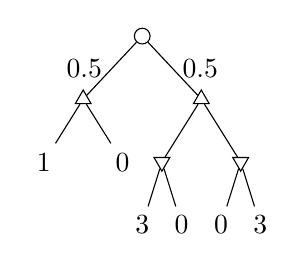
\begin{tikzpicture}
\node [ch] {}
    child{ node [ma] (i1_1) {} 
	    child{ node {1}}
    	    child{ node {0}}
    	    edge from parent node[left] {0.5}
    }
    child{ node [ma] (i1_2) {}
	    child{ node [mi] (i2_1) {}
			   child{ node {3}}
	    		   child{ node {0}}
			 }	    
	    child{ node [mi] (i2_2) {}
			   child{ node {0}}
	    		   child{ node {3}}
			 }
		edge from parent node[right] {0.5}
	};
\end{tikzpicture}
~~~
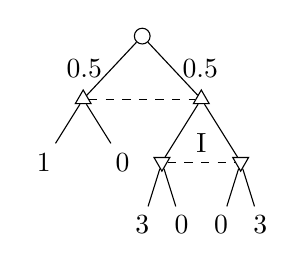
\begin{tikzpicture}
\node [ch] {}
    child{ node [ma] (i1_1) {} 
	    child{ node {1}}
    	    child{ node {0}}
    	    edge from parent node[left] {0.5}
    }
    child{ node [ma] (i1_2) {}
	    child{ node [mi] (i2_1) {}
			   child{ node {3}}
	    		   child{ node {0}}
			 }	    
	    child{ node [mi] (i2_2) {}
			   child{ node {0}}
	    		   child{ node {3}}
			 }
		edge from parent node[right] {0.5}
	};
\draw [dashed] (i1_1) -- (i1_2);
\draw [dashed] (i2_1) -- (i2_2) node[midway, above] {I};
\end{tikzpicture}
\end{center}
\caption{Two example games with maximizing $\bigtriangleup$, minimizing $\bigtriangledown$ and chance $\bigcirc$ players. The game of the left has perfect information, while the game on the right has imperfect information. \label{fig:coordGame}}
\end{figure}

In a \defword{match} (online game), each player is allowed little or no preparation time before playing (preventing the offline advance computation of approximate equilibria solutions).
There is a current \defword{match history}, $\tth$, initially the empty history $\emptyset$ representing the start of the match. Each turn, 
the agent controlling $P(\tth)$ is given $t$ time units to decide on a \defword{match action} $\tta \in A(\tth)$ and the 
match history then changes using $\tth \leftarrow \tth \tta$. There is a single referee who knows $\tth$, samples chance outcomes 
as needed from $\sigma_c(\tth)$, and reveals $I(\tth)$ to $P(\tth)$ on their turn. The players play until the match is terminated, 
giving each player $i$ a payoff of $u_i(\ttz)$.

\subsection{The Problem of Non-Locality}

%Complexities of online search vs. offline equilibrium computation. Notions of subgame perfection (sequential equilibrium). 
%Perfect infromation games. Subject perfection
%Minimax and MCTS are online approximations of backward induction. 
%Explain why this is not the case in imperfect information search. 
%Show what can go wrong if you use a perfect information search method.

Consider the two extensive games depicted in Figure~\ref{fig:coordGame}. The perfect information game on the left can be solved using {\it backward induction}
as follows: the minimizing player has two subgames with value 0 (since $0 < 3$), leading to a value of 0 for the maximizing player's larger subgame. The only other subgame for max gives a value of $1$. Therefore, the expected value of the full game is $0.5 \cdot 1 + 0.5 \cdot 0 = 0.5$.

This pattern of reasoning cannot be applied to the imperfect information game on the right, because changes in strategies affect the expected payoffs of more 
than just a single state and subtree.
The optimal (Nash equilibrium) strategy for the game on the right is obtained by solving $\max_{\sigma_1 \in \Sigma_1} \min_{\sigma_2 \in \Sigma_2} u_1(\sigma_1, \sigma_2)$, which gives $\bigtriangleup$ to play $(\frac{1}{2},\frac{1}{2})$ and for $\bigtriangledown$ to play (left,right) with probabilities ($\frac{1}{3}$,$\frac{2}{3}$). The expected value of the game is $1$.

Current approaches, when given information set $I$, will repeatedly sample and search one of subtrees of states in $I$, aggregating the information collected to make a final recommendation. When hidden information is revealed for search, Russel and Norvig refer to this technique as ``averaging over clairvoyance''~\cite{russellnorvig}. However, even if the information structure is kept intact and information is aggregated during the searches, such as in Information Set Monte Carlo tree search (ISMCTS)~\cite{Cowling12ISMCTS}, the problem still occurs. If subtrees of $I$ are sampled equally often, a searching player will not have any preference between left and right and may recommend $(\frac{1}{2},\frac{1}{2})$. However, mixing uniformly at $I$ is not part of an equilibrium in this game. The payoff to $\bigtriangleup$ for playing right would be $\frac{1}{2} \cdot \frac{3}{2} = \frac{3}{4}$, which would give $\bigtriangleup$ incentive to switch to play left more often (since its expected value is higher), in turn giving $\bigtriangledown$ incentive to deviate. 

Note that sampling uniformly at $I$ corresponds to the proper belief distribution over states in $I$ given optimal play. Therefore, the problem occurs even if subtrees are sampled from the proper belief distribution. 

To overcome this problem, we propose a new approach. Instead of adapting perfect information search techniques to imperfect information games, we present online variants of Monte Carlo equilibrium approximation algorithms that have been successful in the offline setting. 

% Sort of reptitive from non-locality discussion from before

%A perfect information game can be broken down into subgames and solved independently. 
%An equilibrium is called subgame perfect if its portion used in every subgame is also an equilibrium in that subgame. 
%Every perfect information game has a pure subgame perfect equilibrium, which can be found by backward induction. 
%Search algorithms simply aim to identify the single optimal action at the search tree's root. 
%Imperfect information games cannot be easily broken down into subgames. In general, the optimal strategies in an inner 
%information set could be mixed and depend on the probabilities that individual nodes in the information set are 
%reached. These probabilities depend on the strategies of the players in the tree above the information set, which in 
%turn depend on the payoffs obtained from other parts of the tree. 

%Hence, the ``subgames'' cannot be solved independently 
%and the search problem is more complex. 

%Some previous work has been done for accelerating equilibrium computation by solving or approximately solving subgames, particularly 
%in end-game situations~\cite{Gilpin06Competitive,Gilpin07Better,Ganzfried13Endgame}. These techniques tend to help in practice, 
%but as shown in \cite{Ganzfried13Endgame}, non-locality prevents these methods from producing equilibrium strategies in general. 
%Using CFR to solve decomposed subgames has also recently been investigated~\cite{Burch14Solving}. Whether this decomposition 
%could be used in Monte Carlo simulations is an interesting topic of future work.

%\subsection{Information Set Monte Carlo Tree Search}

%The implementation details of ISMCTS described in \cite{Cowling12ISMCTS} have impact on efficiency of the method for various games, but in essence, the multi-observer variant of the algorithm incrementally builds the game tree similarly to MCTS, but it places a multi-armed bandit algorithm at each information set rather than at each state. After a non-root information set is reached during the match, further simulations are run from a random node in this information set with uniform probability. This prevents the algorithm from converging to the optimal solution in the game.
%Consider the game in Figure~\ref{fig:coordGame}.
%Suppose ISMCTS searches from information set $I$. Because utilities for actions taken from both states are combined, ISMCTS will choose left and right action equally often. However, mixing uniformly at $I$ is not part of an equilibrium in this game, since it would lead to an expected utility of $\frac{3}{4}$ to the maximizing player for playing right, which would give an incentive to the maximizer to always play left and in that case, the minimizer would be better off playing right, reaching expected reward of $0.5$.


\subsection{Offline Precomputation of Approximate Equilibria}

Counterfactual Regret (CFR) is a notion of regret at the information set level for extensive-form games~\cite{CFR}. 
The CFR algorithm iteratively learns strategies in self-play, converging to an equilibrium. 
The \defword{counterfactual value} of reaching information set $I$ is the expected payoff given that player $i$ played to reach $I$, the opponents played 
$\sigma_{-i}$ and both players played $\sigma$ after $I$ was reached:
\begin{equation}
\label{eq:cfv}
v_i(I,\sigma) = \sum_{(h,z) \in Z_I} \pi^{\sigma}_{-i}(h) \pi^{\sigma}(h,z) u_i(z), 
\end{equation}
where $Z_I = \{ (h,z)~|~z \in Z, h \in I, h \sqsubset z \}$.
Suppose, at time $t$, player $i$ plays with strategy $\sigma^t_i$. 
Define $\sigma^t_{I \rightarrow a}$ as identical to $\sigma^t$ except at $I$ action $a$ is taken with probability $1$. 
The counterfactual regret of not taking $a \in A(I)$ at time $t$ is $r^t(I,a) = v_i(I,\sigma^t_{I \rightarrow a}) - v_i(I,\sigma^t)$. 
The algorithm maintains the cumulative regret $R^T(I,a) = \sum_{t=1}^T r^t(I,a)$, for every action at every information set of every player. 
Then, the distribution at each information set for the next iteration $\sigma^{T+1}(I)$ is obtained individually using 
regret-matching~\cite{Hart00}. The distribution is proportional to the positive portion of the individual actions' regret:
\begin{equation*}
\label{eq:rm}
\sigma^{T+1}(I,a) = \left\{
\begin{array}{ll}
R^{T,+}(I,a) / R^{T,+}_{sum}(I) & \mbox{if } R^{T,+}_{sum}(I) > 0 \\ 
1 / |A(I)|                   & \mbox{otherwise,}
\end{array} \right.
\end{equation*}
where $x^+ = \max(0,x)$ for any term $x$, and $R^{T,+}_{sum}(I) = \sum_{a' \in A(I)} R^{T,+}(I,a')$. Furthermore, the algorithm maintains for each information set the average strategy profile
\begin{equation}
%\bar{\sigma}^T(I,a) = \frac{1}{T}\sum_{t=1}^T \sigma^t(I,a).
\bar{\sigma}^T(I,a) = \frac{\sum_{t=1}^T \pi^{\sigma^t}_i(I) \sigma^t(I,a)}{\sum_{t=1} \pi^{\sigma^t}_i(I)}, 
\end{equation}
where $\pi^{\sigma^t}_i(I) = \sum_{h \in I}\pi^{\sigma^t}_i(h)$.
The combination of the counterfactual regret minimizers in individual information sets also minimizes the overall average regret \cite{CFR}, and hence the average profile is a $2\epsilon$-equilibrium, with $\epsilon \rightarrow 0$
as $T \rightarrow \infty$.

Monte Carlo Counterfactual Regret Minimization (MCCFR) applies CFR to sampled portions of the games~\cite{Lanctot09Sampling}. 
In the \defword{outcome sampling} (OS) variant of the algorithm, a single terminal history $z\in Z$ is sampled in each iteration. 
The algorithm updates the regret in the information sets visited along $z$ using the 
\defword{sampled counterfactual value}, 
\begin{equation*}
\tilde{v}_i(I,\sigma) = \left\{
\begin{array}{ll}
\frac{1}{q(z)} \pi^{\sigma}_{-i}(h) \pi^{\sigma}(h,z) u_i(z) & \mbox{if } (h,z) \in Z_I\\
0  & \mbox{otherwise,}
\end{array} \right.
\end{equation*}
where $q(z)$ is the probability of sampling $z$. 
As long as every $z \in Z$ has non-zero probability of being sampled, $\tilde{v}_i(I,\sigma)$ is an unbiased estimate of $v(I,\sigma)$ 
due to the importance sampling correction ($1/q(z)$). For this reason, applying CFR updates using these sampled counterfactual values 
on the sampled information sets values also eventually converges to the approximate equilibrium of the game with high probability. 
The required number of iterations for convergence is much larger, but each iteration is much faster.

In Poker, CFR and MCCFR have been used with much success as offline methods 
for pre-computing approximate equilibria in abstract games~\cite{CFR,Johanson12CFRBR}; the same general 
approach has also been used in Liar's Dice~\cite{Neller11,Lanctot12IR}. 
%additional optimizations that can be applied in Liar's Dice~\cite{Neller11}.
%Essentially, CFR takes time (weeks?) {\it pre-computing} 
%approximate equilibria on abstract poker games, which are then used to look up actions when a decision needs to be made during play. 


\section{Online Outcome Sampling}

%Information set targeted search. Epistemic depth.
%Convergence theorems. Algorithm description.
%Recall outcome sampling (OS) from Section~\ref{sec:cfr}. 

When outcome sampling is used in the offline setting, data structures for all information sets are allocated and created 
before the first iteration starts. In each iteration, every information set that is sampled gets updated. 
% MarcL: these are too strong and kind of miss the point, at least the way they were phrased..
%In the online setting, this is not practical. The limited computation time often does not allow even a single visit of each 
%information set in the game tree. Moreover, the information sets far from the tree root will likely have only very few visits, 
%making the statistics stored in these information sets practically useless. 

We make two essential modifications to adapt outcome sampling to the online search setting.

{\bf Incremental Game Tree Building.} Before the match begins, only the very first (root) information set is added to memory. 
In each iteration, a single information set (at most) is added the information set tree (memory) each iteration.
In particular, when an information set is reached that is not in memory, it is added to memory and then a default 
playout policy (\eg uniform random) takes over for the remainder of the simulation.
Along the playout portion (tail) of the simulation, information sets are not added to memory nor updated.
Along the tree portion (head) of simulation, information sets are updated as normal. 
This way, only the information sets with relevant statistics will be stored in the memory.
%We call this modification \defword{playout-based outcome sampling}

{\bf In-Match Search Targeting.}
%ime per move, the match can after a few moves easily 
%reach a history $\tth$ in an information set that was visited in only a few iterations or even not present in the memory at all.
%The strategy suggested by the algorithm in such an information set can be completely arbitrary.
Suppose several moves have been played since the start of the match leading to $\tth$. 
Plain outcome sampling would continue to sample from the root of the game (not the current match history $\tth$), entirely 
disregarding the region of the game space that the match has headed toward. 
Hence, the second modification we propose is directing the search towards the histories that are more likely to occur during the match currently played.
%Online Outcome Sampling (OOS) builds on playout-based OS by proposing two different ways to direct the search when starting with a particular non-empty match history, $\tth$. 
Note that this history is typically unknown to the players, who know only their information sets it leads to. 
Furthermore, unlike in ISMCTS, OOS always runs samples form the root of the game tree, even with non-empty match history.

We now describe two specific targeting methods.

\subsection{Information Set Targeting (IST)}

Suppose the match history is $\tth$. IST samples histories reaching the current information set ($I(\tth)$), 
i.e., $(h,z) \in Z_{I(\tth)}$, with higher probability than other histories.
The intuition is that these histories are particularly 
relevant since the searching player {\it knows} that one of these $z$ will describe the match at its completion. 
However, focusing fully only on these histories may cause problems, since convergence guarantees are lost.
Consider again the game in Figure~\ref{fig:coordGame}. 
If the minimizing player knows it is in the information set $I$ and focuses all its search only to this information set for sufficiently long, she computes the uniform strategy, which is optimal in the right (coordination) part of the game.
However, if the minimizing player plays uniformly, the maximizing player prefers to switch to always play the left action to increase its payoff in case of not playing the coordination game. Any fixed non-zero probability of sampling the left chance action will 
eventually solve the problem. The regrets are multiplied by the reciprocal of the sampling probability; hence, they influence the strategy 
in the information set proportionally stronger if the samples are rare. 

Note that previous methods, such as PIMC and ISMCTS, {\it always} target $I(\tth)$, \ie with probability 1, and do not 
update predecessors of $I(\tth)$. In contrast, in IST {\it all} information sets in memory reached during each iteration requires updating 
to ensure eventual convergence to an equilibrium.

%What IST does is similar to what previous methods, such as PIMC and ISMCTS, do. However, there some important subtleties

%It is tempting to set $\delta_I$ high. The problem, however, is that 
%focusing too much on $Z_{I(\tth)}$ could 
%have the effect of revealing private information to the opponent. 
%\vlnote{I agree this holds for Exp3-based MMCTS-like approaches, but I do not think it is true for MCCFR. Can you create a simple counter-example as above?} To see this, imagine the subgame 
%defined by placing a single chance node over the histories $h \in I(\tth)$, whose distribution is obtained by previous chance event outcomes. 
%The equilibrium strategy for the opponent in this subgame plays as if the opponent knows the searching player's private information. Therefore,
%we expect that the optimal value of $\delta_I$ will depend on the importance of the hidden information.

\subsection{Public Subgame Targeting (PST)}

A \defword{public action} is an action in the ``public tree'' defined in \cite{12aamas-pcs}. Informally, an action is said to be public if it is observable by all players (e.g., bids in Liar's Dice and bets in Poker are public). Formally, an action $a$ is public, iff 
$\forall i, \forall I \in \cI_i, \forall h_1,h_2\in I: a\in h_1 \Leftrightarrow a\in h_2$.
For example, the extensive-form version of Rock, Paper, Scissors has two information 
sets $I_1 = \emptyset$ and $I_2 = \{ r, p, s \}$; it has no public actions, because each history in 
$I_2$ contains a single unique action (the unobserved ones taken by the first player).  

%a sequence of legal actions from I to I', S(I,I'), is said to be a ``public action sequence'' if every two histories h,h' \in I: hL \in I' and h'L \in I' and S(I,I') describes a one-to-one correspondence between histories in I and histories in I'. A public action, a \in A(I), is one such that every sequence containing a as the first action, S(I,I') = a S(I'',I') where I' is a successor of I is a public action sequence. 

Given a history $h$, let $p(h)$ be the sequence of public actions along $h$ in the same order that they were taken in $h$. 
Define the \defword{public subgame} induced by $I$ to be the one whose terminal history set is
\[Z_{p,I(h)} = \{(h',z)~|~z \in Z, h' \in H, p(h') = p(h), h' \sqsubset z \}.\]
Now, suppose the match history is $\tth$.
Public subgame targeting samples $z \in Z_{p,I(\tth)}$ with higher probability than terminal histories outside this set.

A public subgame then, contains all the terminal histories consistent with the bidding sequence played over the match and
each combination of private chance events for both players. So, in a game of two-player limit Texas Hold'em poker, suppose 
first player bets and second player calls, and then flop is revealed. At this point, the public actions are: bet, call. 
The public subgame described by $Z_{p,I(h)}$ contains every terminal history (including every combination of private chance 
outcomes for all players) with at least two public actions, whose first two public actions are: bet, call.  

%Suppose $\delta_{p,\tth}$ is the probability that any $z$ in this set is sampled. 
%Again, it is tempting to sample from this set with $\delta_{p,\tth} = 1$. 
%However, this is also problematic because the probabilities to reach $\tth$ play a critical role in the convergence in the full game. 
%Nonetheless, the intuition is to spend more time in parts of the tree that are relevant given the progression of the match. Unlike 
%information set targeting, public subgame targeting should not reveal anything about private information. 

\subsection{Algorithm}

\begin{algorithm2e}[t]
  OOS$(h, \pi_i, \pi_{-i}, s_1, s_2, i)$: \; 
  \pushline
  \If{$h \in Z$}{
    \breturn $(1, \delta s_1 + (1-\delta)s_2, u_i(z))$\; \label{alg:terminal}
  }
  \ElsIf{$P(h) = c$}{
    Sample an outcome $a$ and let $\rho_1,\rho_2$ be its probability in targeted and untargeted setting \; \label{alg:chancesample}
    \breturn OOS$(ha, \pi_i, \rho_2 \pi_{-i}, \rho_1 s_1 , \rho_2 s_2, i)$ \;
  }
  $I \gets $ getInfoset$(h, P(h))$ \;
  Let $(a,s_1',s_2') \leftarrow $ Sample$(h, I, i, \epsilon)$ \; \label{alg:sample}
  \If{$I$ is not in memory}{ 
    Add $I$ to memory \;
    $\sigma(I) \leftarrow \mbox{Unif}(A(I))$ \;
    $(x, l, u) \gets $ Playout$(ha, \frac{\delta s_1 + (1-\delta)s_2}{|A(I)|})$ \; \label{alg:playout}
  }
  \Else{
    $\sigma(I) \gets $ RegretMatching$(r_I)$ \;
    $\pi_{P(h)}' \gets \sigma(I,a)\pi_{P(h)}$ \;    \label{alg:newreaches1}
    $\pi_{-P(h)}' \gets \pi_{-P(h)}$ \;             \label{alg:newreaches2}
   % $(\pi_i', \pi_{-i}') \leftarrow$ NewReachProbs$(h, \pi_i, \pi_{-i}, i)$ \;  \label{alg:newreaches}
    $(x, l, u) \gets$ OOS$(ha, \pi_i', \pi_{-i}', s_1', s_2', i)$ \;  
  }
  $c \gets x$ \;                   \label{alg:suffix1} 
  $x \gets x \sigma(I,a)$ \;     \label{alg:suffix2}
  \For{$a' \in A(I)$}{   
    \If{$P(h) = i$}{
      $W \gets u \pi_{-i}~/~l$ \;
      \If{$a' = a$}{
        $r_I[a'] \gets r_I[a'] + (c - x)W$ \;
      }
      \Else{
        $r_I[a'] \gets r_I[a'] - xW$ \;
      }
    }
    \Else{
      $s_I[a'] \gets s_I[a'] + \frac{1}{\delta s_1 + (1-\delta)s_2} \pi_{-i} \sigma(I,a')$ \;  \label{alg:avgstrat}
    }
  } 
  \breturn $(x, l, u)$ \;   \label{alg:returnend} 
  \popline
  \vspace{0.1cm}
  \caption{Online Outcome Sampling. \label{alg}}
\end{algorithm2e}

The algorithm is iterative and samples a single trajectory from the root $\emptyset$ to some 
terminal history. At each information set in memory, $I$, there are two tables maintained: $r_I$ stores cumulative 
regret for each action $a \in A(I)$, and $s_I$ stores the cumulative average strategy probability of each 
action. 

Depending on the targeting method that is chosen (IST or PST), $Z_{sub}$ is one of $Z_{I(\tth)}$ or $Z_{p,I(\tth)}$. 
The pseudo-code is presented as Algorithm~\ref{alg}. 
Each iteration is represented by two calls of OOS where the update player $i \in \{1,2\}$ is alternated. 
Before each iteration, a {\it scenario} is decided: 
with probability $\delta$ the iteration targets the subgame and chooses $z \in Z_{sub}$
and with probability $(1-\delta)$ the usual OS sampling determines $z \in Z$. 
The first parameter of OOS is the current history. 
The next two are strategy's reach probabilities for the update player $i$ and the opponent. 
The third and fourth parameters are overall probabilities that the current sample is generated, one for each scenario: first the targeted and then the untargeted.
The last is the update player. Initial calls have the form OOS$(\emptyset, 1, 1, 1, 1, i)$.  
For the return values, $x$ is a suffix/tail reach probability for both players, 
$l$ is the root-to-leaf sample probability, and $u$ is the payoff of the trajectory in view 
of the update player. 

In outcome sampling, an $\epsilon$-on-policy sampling distribution used at each information set
is defined as 
\begin{equation*}
\label{eq:ossample}
\Phi(I,i) = \left\{
\begin{array}{ll}
\epsilon \cdot \mbox{Unif}(A(I)) + (1-\epsilon)\sigma_i(I) & \mbox{if } P(I) = i\\ 
\sigma_i(I)                                          & \mbox{otherwise,}
\end{array} \right.
\end{equation*}
and denote $\Phi(I,i,a)$ the probability of sampling $a \in A(I)$. 

The sampling at chance's choices on line~\ref{alg:chancesample} depends on the method and the scenario being used. For example, when using information set targeting, the outcome that is sampled must be consistent with match history.

A critical part of the algorithm is the action chosen and sample reach updates on line~\ref{alg:sample}. If $I$ is not in memory, then an action is sampled uniformly. Otherwise, in the targeted scenario, the current history $h$ is always in the targeted part of the game and an action from $\{a~|~\exists z\in Z \; (ha,z)\in Z_{sub}\}$ is selected using the distribution $\Phi(I(h),i)$ normalized to one on this subset of actions. If we define $sum=\sum_{(ha,z)\in Z_{sub}}\Phi(I,i,a)$ then $s_1' = s_1\Phi(I,i,a)/sum$. In the untargeted scenario, any action $a \sim \Phi(I,i)$ can be sampled. If the action is not leaving the targeted part of the game (i.e., $(ha,z)\in Z_{sub}$) then $s_1' = s_1\Phi(I,i,a)/sum$ otherwise $s_1'=0$. In all cases $s_2' = \Phi(I,i,a) s_2$.

These sample reach probabilities are combined into one at a terminal history on line~\ref{alg:terminal}, 
start of the playout on line~\ref{alg:playout}, and when updating the average 
strategy on line~\ref{alg:avgstrat}. 

%In practice, the algorithm does not sample $z \in Z_{sub}$ directly, but rather on a per-action basis. 
%There are two stages, the prefix stage ($h \sqsubset \tth$), and the tail stage (either $\tth \sqsubseteq h$ or $h$ is 
%off the match path). 
%In the prefix stage, $\cP_{sub}$ is a distribution 
%that assigns some high probability $\gamma$ to sampling an action that is consistent with $\tth$. In the tail case, the 
%sampling distribution is $\epsilon$-on-policy, so action $a \in A(I)$ is sample with probability 
%$\epsilon/|A(I)| + (1-\epsilon)\sigma(I,a)$. Also, no exploration is done on opponent histories, so $\epsilon = 0$ when 
%$P(h) = -i$.

The playout on line~\ref{alg:playout} samples to the end of the game with some playout policy at each step; we use uniform random, 
but in general one could use a informed policy based on domain knowledge as well. 
Unlike MCTS, the playout policy in OOS must compute $l$ when reaching a terminal and update the tail probability $x$ when returning
as done on line~\ref{alg:suffix2}. Lines~\ref{alg:newreaches1} and \ref{alg:newreaches2} modify $P(h)$'s reach probability 
by multiplying it by $\sigma(I,a)$, keeping the other value the same.

%Lines~\ref{alg:suffix1} to \ref{alg:returnend} % second ref does not seem to work
Lines~\ref{alg:suffix1} to 24
contain the usual outcome sampling updates. Note that regrets are updated at the 
update player histories, while average strategy tables at opponent histories. 
%\mlnote{Still need to add some more detail to 
%earlier sections so that this last part is not too confusing.}

\begin{theorem}
Let $\bar{\sigma}^t_m(\delta,\tth)$ be a strategy produced by OOS with scheme $m \in \{ \mbox{IST}, \mbox{PST} \}$ 
using $\delta < 1$ started from $\tth$ run for $t$ iterations, with exploration $\epsilon > 0$.  
For any $p \in (0, 1], \varepsilon > 0$ there exists $t < \infty$ such that with 
probability $1-p$ the strategy  $\bar{\sigma}^t_m(\delta,\tth)$ is a $\varepsilon$-equilibrium strategy. 
\label{thm:consistency}
\end{theorem}
Since every terminal history has non-zero probability of being sampled, eventually every information 
set will be contained in memory. Then, the algorithm becomes MCCFR with a non-uniform sampling scheme.
Consequently by \cite[Theorem 5]{Lanctot09Sampling} OOS minimizes external regret with high probability.

Note that due to non-locality, this consistency property cannot hold generally for any search 
algorithm that does not modify $\sigma(I)$ at previous $I(h)$ such that $h \sqsubset \tth$. However, 
it is an open question as to whether any of the previous algorithms could be modified to ensure 
consistency.

\section{Empirical Evaluation}

%\mlnote{This section is still quite rough. I've commented out much of the text for now.}

%Here are some ides for what we could look at empirically: 
%\begin{itemize}
%\item Compare sampling techniques in each domain
%\item Quality of OOS as a function of the length of the match history $\tth$ (and time limits?)
%\item Robustness/sensitivity of $\delta_I$ and $\delta_{I,\tth}$ with observed convergence,
%\item Importance of ``retaining the tree'' from previous searches along the same match $z$ (suspected to be high)
%\item Performance comparisons (win rates and exploitability) between sampling techniques and some state-of-the-art
%algorithms in imperfect information search (ISMCTS, PIMC, MMCTS), 
%possibly also show exploitation / exploitability trade-offs as in RNash work
%\item (probably too much for this one paper) What if there are a sequence of multiple matches and we can reuse computation from 
%previous matches? 
%\item How does the story change with or without \{ incremental tree-building, targeting, retaining memory between searches \}
%\end{itemize}
%
% How does the story change: 
% - with/without targeting (as a function of delta)
% - with/without incremental tree-building
% - with/without remembering between moves

We now compare the head-to-head performance and exploitability 
of OOS and ISMCTS on two games. % with different sources of imperfect information. 
%We show the effects of targeting methods and $\delta$ values. 
%We start by describing each game, whose utilities are in $\{-1, 0, 1\}$. 

Liar's Dice, LD($D_1$,$D_2$), also known as Dudo, Perudo, and Bluff is a dice-bidding game. 
Each die has six sides with faces \epsdice{1} to \epsdice{5} and a star $\star$. 
Each player $i$ rolls $D_i$ of these dice and looks at them without showing them to their opponent. 
Each round, players alternate by bidding on the outcome of all dice in play until one player ``calls liar'', 
\ie claims that their opponent's latest bid does not hold.
A bid consists of a quantity of dice and a face value.  
A face of $\star$ is considered wild and counts as matching any other face.
To bid, the player must increase either the quantity or face value of the current 
bid (or both). The losing player discards a number of dice equal to how many dice were missing 
to have a valid bid. The players continue until one player has no more dice.

Imperfect Information II-Goofspiel($N$) is a two-player card game where each player is
given a private hand of bid cards with values $1$ to $N$. A different
deck of $N$ point cards is placed face up in a stack 
On their turn, each player bids for the top point card by 
choosing a single card in their hand. 
The highest bidder gets the point card and adds the point total to their score, discarding
the points in the case of a tie. 
This is repeated $N$ times and the winner is the player with the highest score.
In, II-Goofspiel the players only discover who won or lost a bid but not the bid cards played.
Also, we assume the point-stack is strictly increasing: 1, 2, $\ldots N$.

%Phantom Tic-Tac-Toe (PTTT) is played on a 3-by-3 board, 
%initially empty, where the goal is to claim three squares along the same row, column, or diagonal. 
%However, in PTTT, players' actions are private. 
%Each turn, a player attempts to take a square of their choice. 
%If they fail due to the opponent having taken that square on a previous turn, the same player 
%keeps trying to take an alternative square until they succeed. 
%Players are not informed about how many attempts the opponent made before succeeding. 
%The game ends immediately if there is ever a connecting line of squares belonging to the same player. 
%The winner receives a payoff of $+1$, while the losing player receives $-1$. 

We will focus our experiments on LD(1,1) and II-Goofspiel(6). While these games are considered small by 
search algorithm standards, it is still possible to compute best response strategies to measure exploitability, 
allowing us to show the observed convergence of the strategies
produced by OOS. We include preliminary results in LD(2,2). 

To improve performance against irrational play, we use a more explorative regret matching, 
$\sigma^{T+1}_\gamma(I,a) = \gamma/|A(I)| + (1-\gamma) \sigma^{T+1}(I,a)$, with $\gamma = 0.01$. 
While this could effect convergence, we observe in our experiments that exploitability 
decreases as search time increases.  

\subsection{Head-to-Head Performance versus Exploitability} 

\begin{figure}[t!]
\begin{center}
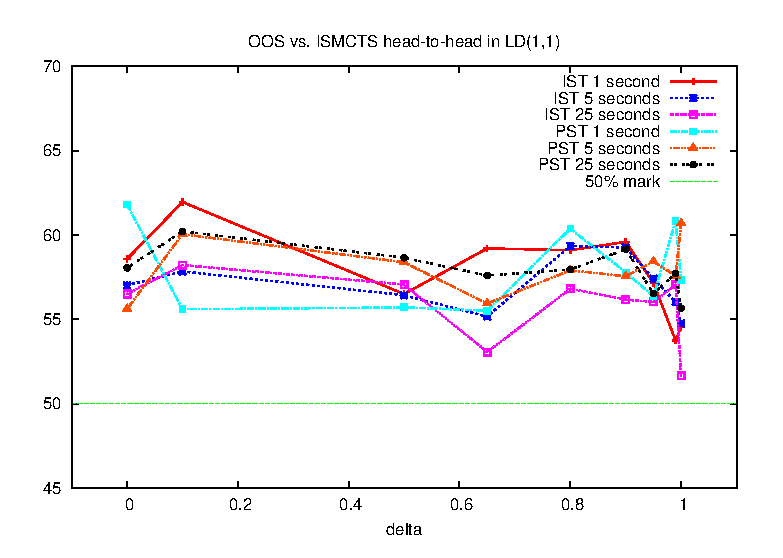
\includegraphics[scale=0.55]{plots/ismcts-oos-perf} \\
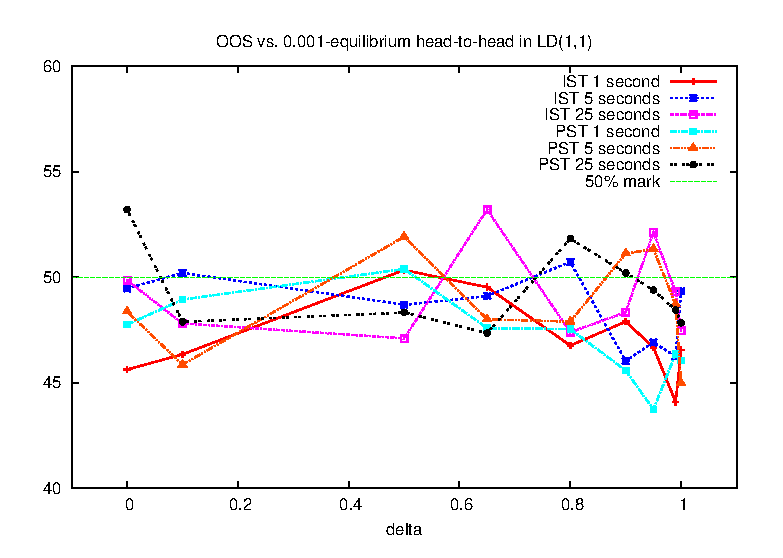
\includegraphics[scale=0.55]{plots/eq-oos-perf} \\
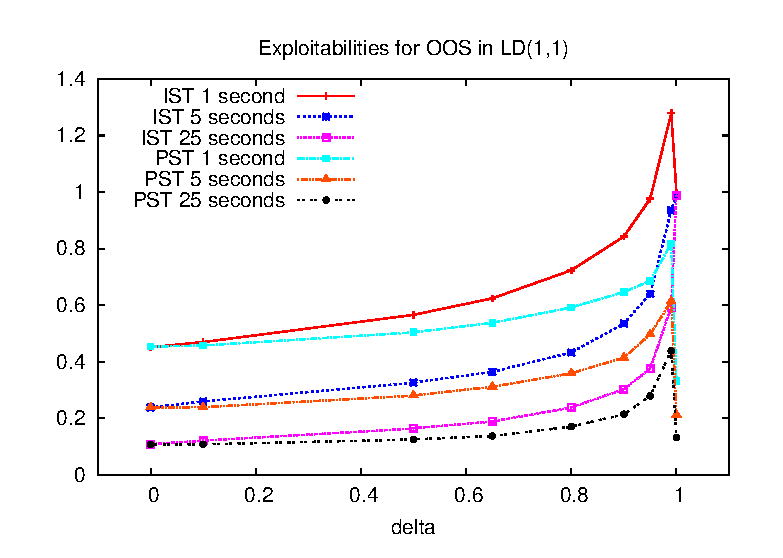
\includegraphics[scale=0.55]{plots/oos-expl} \\
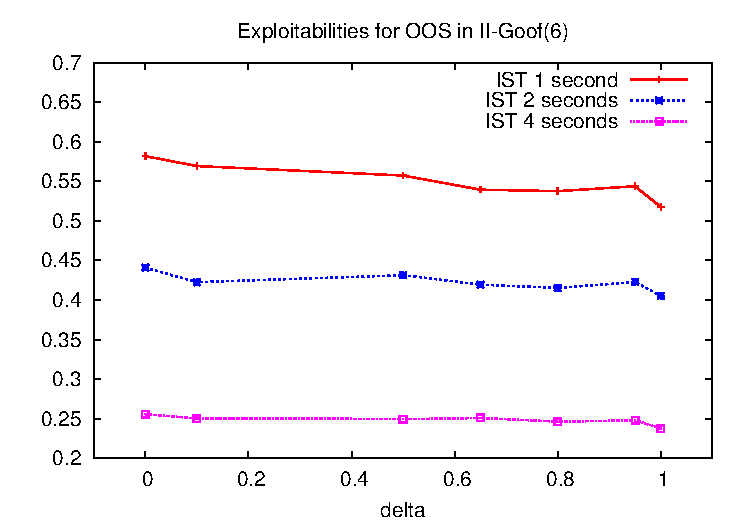
\includegraphics[scale=0.55]{plots/goof-expl} \\
\caption{Results for OOS in LD(1,1). From top: win rate (\%) of OOS vs. ISMCTS, win rate (\%) of 
OOS vs. a 0.001-equilibrium, approximate $\epsilon_{\sigma}$ using aggregate method in LD(1,1) 
and II-Goofpiel(6).  }
\label{fig:results}
\end{center}
\end{figure}

%Here are some first results for performance and/or exploitability analysis of the algorithms. 
%Note that unless otherwise stated, memory is retained and not cleared between successive searches
%(which has no effect in ISMCTS).
%\mlnote{I have played against the ISMCTS strategy and I believe it's converging to a particular 
%pure (and bad) strategy.}

%We evaluate head-to-head performance by simulating several games of each algorithm against the other
%and counting wins and losses. 

In games like Poker and Liar's Dice, it is often critical to play in such a way that the opponent 
cannot easily infer the private information. This explains partly why CFR-based methods have 
enjoyed so much success in the offline approach. 
In the online setting, however, since the tree is built incrementally, only partial strategies
are produced. 
We are unaware of any methods for assessing the worst-case exploitability of strategies 
produced by an online search algorithm. 
We therefore propose two new methods to approximate the exploitability of the produced strategies. 

In the offline setting, measuring exploitability can be done by a recursive walk of the game 
tree using expectimax. In online search, the algorithm computes only 
a partial strategy. 
The first \defword{full stitching} method 
enumerates each $I \in \cI_i$ in topologically-sorted order starting at the root, 
%tries to capture as closely as possible the distributions that would be computed 
%for each $I$ if they were reached in a match: 
running a search from $I$ re-using only the information computed in previous searches from ancestors of $I$, saving the 
distribution computed at $I$, and passing down the state of memory only for children of $I$. 
We do not save changes made to ancestors when searching at $I$ to ensure 
a fair comparison between OOS and ISMCTS. Full stitching provides the best representation of a full strategy
that would eventually be produced by OOS since it builds distributions at each information set in the 
same way as OOS would if they were reached during play.
However, full-stitching requires $|\cI|$ searches and memory, which is impractical on large games. 

We also propose a the multi-match \defword{aggregate method}. 
This method first creates a global (accumulating) strategy data structure for each player type and generates a 
set of matches $M$. Then, each $m \in M$ is simulated invoking the appropriate search algorithm at each observed 
$I$ along $m$. 
Since $m$ is predetermined, the choice made by the search algorithm is discarded, but the information computed 
(visit counts in ISMCTS, $s_I$ in OOS) is added into the global strategy data structure belonging to the player
who searched. 
For a fair comparison, the first $I$ reached along each $m$ aggregates all the information gained in the search 
but for future $I'$, only the information collected in each $I''$ reachable by $I'$ is aggregated.
Note that it is safe to combine the information in this way: in ISMCTS the actions chosen and visits are independent of 
how $I'$ was reached. In OOS, the accumulating $s_I$ values of two converging $\epsilon$-equilibrium average 
strategies can be combined due to linearity of expected utility. 

%a the \defword{partial stitching} method which does the same as full stitching to a fixed depth from the root, except also 
%retains values from children information sets reached by the searches started along the frontier of the depth limit.
% Probably will ditch this single-match method when partial stitching is working.
%And the \defword{single-match} method: this simply runs several matches and saves all values from each $I$ searched (as well as all of its reachable
%children information sets) search, overwriting previously saved values as necessary. 
 

In our experiments ISMCTS uses $C = 2$; tuning shows that the $C$ value does not 
affect the performance. 
In II-Goofspiel(6) we run searches for 1, 2, and 4 seconds.
As there are no public actions, we only compare IST in II-Goofspiel. 
Over a range of values for $\delta$ and all time settings, there was no statistically significant
winner in head-to-head matches between IST and ISMCTS. 
Exploitability is shown in Figure~\ref{fig:results}. 
For reference, the exploitability values of ISMCTS was 0.95, 0.96, 0.91 for search times of 
1, 2, and 4 seconds. We observe that exploitability generally 
decreases as search time increases and changes little as $\delta$ increases, with its 
lowest points at $\delta = 1$. 
This result was surprising, and we suspect it is due OOS benefiting from the reuse of 
values from previous searches in the same match. 

In LD(1,1), we try searches for 1, 5, and 25 seconds. 
When played against a uniform random player, among all values for delta and time settings, 
IST wins 79.2-86.7\% and PST wins 78.6-84.0\%, with a non-noticeable differences across $\delta$ values. 
ISMCTS beat uniform random 79.8-82.4\% at 1, 5, and 25 seconds. 
Upon further inspection, ISMCTS very quickly converges to the same strategy every time: as first player, 
with a weak roll ($r = \epsdice{1}, \epsdice{2},$ or \epsdice{3}) it bids 2-$r$ in the hope that by chance the
opponent has the same roll because if it did not, the second player would have a winning response most of the time.
On a roll of $r = \epsdice{4}$ or $r = \epsdice{5}$ it always bids 1-$r$ because it wins most of time. Either way, as 
second player ISMCTS selects responses based on the same reasoning, inducing the first player's roll based on their
first bid. This also explains the relative exploitability values in Table~\ref{tbl:fullstitching}: the first player
plays overly safely and hence is hard to exploit, meanwhile the second player best-responds to an expected pure first 
player strategy, which makes it highly exploitable. 
Our exploitability experiments shows a similar skewed first vs. second player effect in II-Goofspiel. 

Results for OOS variants on LD(1,1) are shown in Figure~\ref{fig:results}. Firstly, in head-to-head performance 
we notice OOS wins 55-60\% of games against ISMCTS, results for $\delta \in \{ 0.1, 0.8, 0.9 \}$ seem somewhat 
consistent across variants and time settings, with varied effects for $\delta > 0.9$. 
Against the 0.001-equilibrium strategy, 
$\delta = 0.5, 0.65$ seems the most robust across variants and time settings, with varied effects when $\delta > 0.9$.
Exploitability of ISMCTS strategies computed by the multi-match method was 0.88, 0.82, 0.79 at search times of 
1, 2, and 25 seconds. There are some clear trends for the exploitability of OOS strategies. 
First, there is an observed decrease in exploitability as time increases, independent of $\delta$. 
When $\delta$ is varied at the same time setting, the exploitability of the global strategy increases with $\delta$. 
Then, when $\delta = 1$ every time setting for IST converges to the same highly-exploitable point, illustrating the 
theoretical problems with full targeting manifesting in practice. 
Interestingly, this is not the case for PST, where $\delta = 1$ is actually always the best-case scenario. 
In Liar's Dice, this is sensible because there is no reason to believe that any histories outside the public subgame 
will effect the decisions being made when in the public subgame. 
The sudden drop from $\delta = 0.99$ to $1$ could be caused by the fact that as $\delta$ increases the 
variance of the importance-sampling corrections of the off-match samples grows; when $\delta = 1$ the 
sampled counterfactual values may be biased, but have much lower variance. 
PST is less affected than IST by the targeting and appears to have lower exploitability. 
For each method and all values of $\delta$: increasing the search time decreases exploitability. 
The exploitability values from Table~\ref{tbl:fullstitching} also show this trend. 

We performed one head-to-head experiment consisting of 500 games of PST($\delta = 0.8$) vs. ISMCTS, in LD(2,2)
with 25 seconds of search time per move. 
PST won 256 games, showing a competitive promise on 
this much larger game with roughly 352 million information sets. 

%Finally, inspired by~\cite{Auger11Multiple}, we started an initial investigation of OOS and ISMCTS in Phantom Tic-Tac-Toe. 
%We noticed that the mixed distribution obtained by normalizing the visit counts of ISMCTS was producing a 
%similar distribution as OOS on the second-player's first action. As in the Rock, Paper, Scissors
%example~\cite{Shafiei09}, we designed a biased version that gave higher payoff if the final line 
%included a side. This modification led to OOS and ISMCTS producing two distinctly different distributions at the second 
%player's first action. 

\begin{table}
{\small
\begin{center}
\begin{tabular}{ccccc}
Algorithm     & Time & $\epsilon_1$ & $\epsilon_2$ & $\epsilon_\sigma$ \\
\hline
ISMCTS        & 1s   & 0.235  & 0.574  & 0.808 \\
IST           & 1s   & 0.337  & 0.311  & 0.648 \\
PST           & 1s   & 0.203  & 0.211  & 0.414 \\
\hline
ISMCTS        & 5s   & 0.251  & 0.548  & 0.799 \\
IST           & 5s   & 0.229  & 0.295  & 0.524 \\
PST           & 5s   & 0.148  & 0.125  & 0.273 \\
\hline
\end{tabular}
\caption{LD(1,1) exploitability using full-stitching, $\delta = 0.9$.} 
\label{tbl:fullstitching}
\end{center}
}
\end{table}


\section{Conclusion}

In the paper, we have introduced Online Outcome Sampling, the first Monte Carlo 
Tree Search algorithm that is guaranteed to produce  
approximate equilibrium strategies as search time per move is increased in imperfect information games.
We showed that in head-to-head performance, OOS is able to compete with 
ISMCTS while producing strategies with lower exploitability
at the same search time in Liar's Dice and II-Goofspiel.
We propose two methods for targeting relevant parts of the game based on the current match history, 
IST and PST.
In II-Goofspiel, results are only slightly affected by different targeting probabilities, whereas the
effect is stronger in LD(1,1), with PST seeming better overall.

In future work, we hope to investigate more and larger games such as 
no-limit poker, and the effect of informed playout policies. 
Ultimately, we want to make practical comparisons to other 
baseline algorithms such as 
PIMC~\cite{Long10Understanding}, MMCTS~\cite{Auger11Multiple}, and IIMC~\cite{Furtak13Recursive}.
One interesting question is whether the subgame decomposition ideas of~\cite{Burch14Solving} could be 
adapted to the online search setting. 
Finally, using MCRNR~\cite{Ponsen11Computing} as the base algorithm could provide a balance between 
exploitability and exploitation against known opponents.

\vspace{0.2cm}

{\small \noindent {\bf Acknowledgments.} This work is partially funded by the Netherlands Organisation for Scientific 
Research (NWO) in the framework of the project Go4Nature, grant number 612.000.938 and the Czech 
Science Foundation, grant no. P202/12/2054.}

\bibliographystyle{aaai}
\bibliography{iioos}

\end{document}



